\section{\agb\, Candidate Distribution}
\label{sec:distribution}
%Introduce the section. What's the overall gist? What are the high-level details that define this section? You show the full candidate distribution throughout the galaxy as well as in color-color space. You use OGLE AGB stars to define O- and C-rich AGB star color-magnitude trends as a basis for calculating the distances to AGB stars
Having obtained our candidate sample, we validate by observing the spatial distribution of candidate AGB stars throughout the sky. We begin with the distribution of candidates in latitude and longitude, as well as their distributions in notable color-color relationships. Because their NIR brightness is dictated chiefly by the temperatures and compositions of their substantial dusty circumstellar shells, which themselves occupy a narrow range of potential temperatures, we can use their color information and narrow magnitude distribution to produce a color-magnitude relationship for AGB stars and estimate their distances. 

We set that stage using known chemically-classified AGB stars from OGLE in the magellanic clouds and find that narrow color-magnitude relationship. We then extend that relationship to our candidate sample, and continue on to produce a three-dimensional map of the galaxy in AGB stars. We discuss the methods involved in that production, the limitations of those methods, and the resulting galactic density distribution of our candidate AGB sample.

\subsection{The Full Candidate Distribution}
%Talk about the full distribution in galactic latitude and longitude space. Talk about how the distribution in color-color space is different depending on the region of the galaxy being explored. Where are the majority of stars located in physical space? Color-color space? Any trends worth noting outside of hard boundaries imposed by color cuts? This does not have to be a significantly long section, this is just a description of the data.
We divide the candidate sample into 6 regions based on galactic position and investigate the resulting galactic and color-color distributions. These distributions can be seen in figures~\ref{fig:color_map_candidates0} through ~\ref{fig:color_map_candidates5}. The positional breakdown of the spatial regions are in Table~\ref{tab:region_table}:

\begin{table}[h]
	\begin{center}
	\scalebox{0.85}{		
		\begin{tabular}{c l r r}
		\hline\hline
		Region & Description & Count\\
		\hline
		1 & $\lvert\text{gal } b \rvert > 5$, $r_\text{GC} > 20$ & 22,280\\
		2 & $\lvert\text{gal } b \rvert < 5$, $r_\text{GC} > 20$, $\lvert\text{gal } l \rvert < 90$ & 165,886\\
		3 & $\lvert\text{gal } b \rvert < 5$, $r_\text{GC} > 20$, $\lvert\text{gal } l \rvert > 90$ & 52,715\\
		4 & $r_\text{GC} < 20$, $r_\text{GC} > 10$ & 37,364\\
		5 & $r_\text{GC} < 10$, $r_\text{GC} > 3$ & 18,856\\
		6 & $r_\text{GC} < 3$ & 2,861\\
		\hline\hline
		\end{tabular}
		}
	\caption{$r_\text{GC}$ is the radius from the Galactic center in degrees. \label{tab:region_table}}
	\end{center}
\end{table}



What we find is that, regardless of location, Galactic AGB candidates primarily populate the region of W1-W2 vs W2-W3 occupied by O-rich OGLE AGB stars with W1-W2 $<$ 0.4. Additionally the inner 5 kpc contains most of the candidate AGB stars, with 240,881 candidates outside of 20$^\circ$ from the Galactic  center.
\begin{figure}[h]
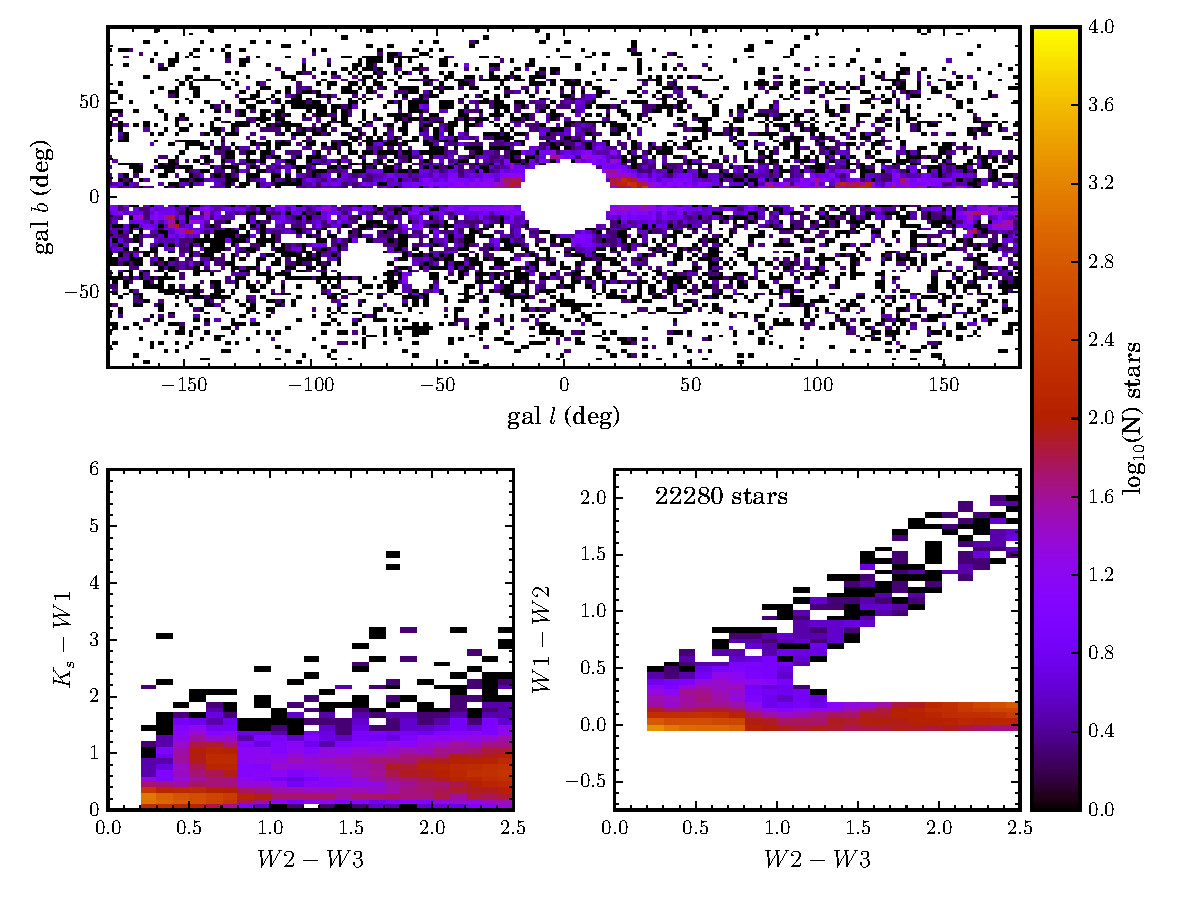
\includegraphics[width=6.5in]{figs/color_and_map_candidates_region0.pdf}
\caption{\label{fig:color_map_candidates0}}
\end{figure}

\begin{figure}[h]
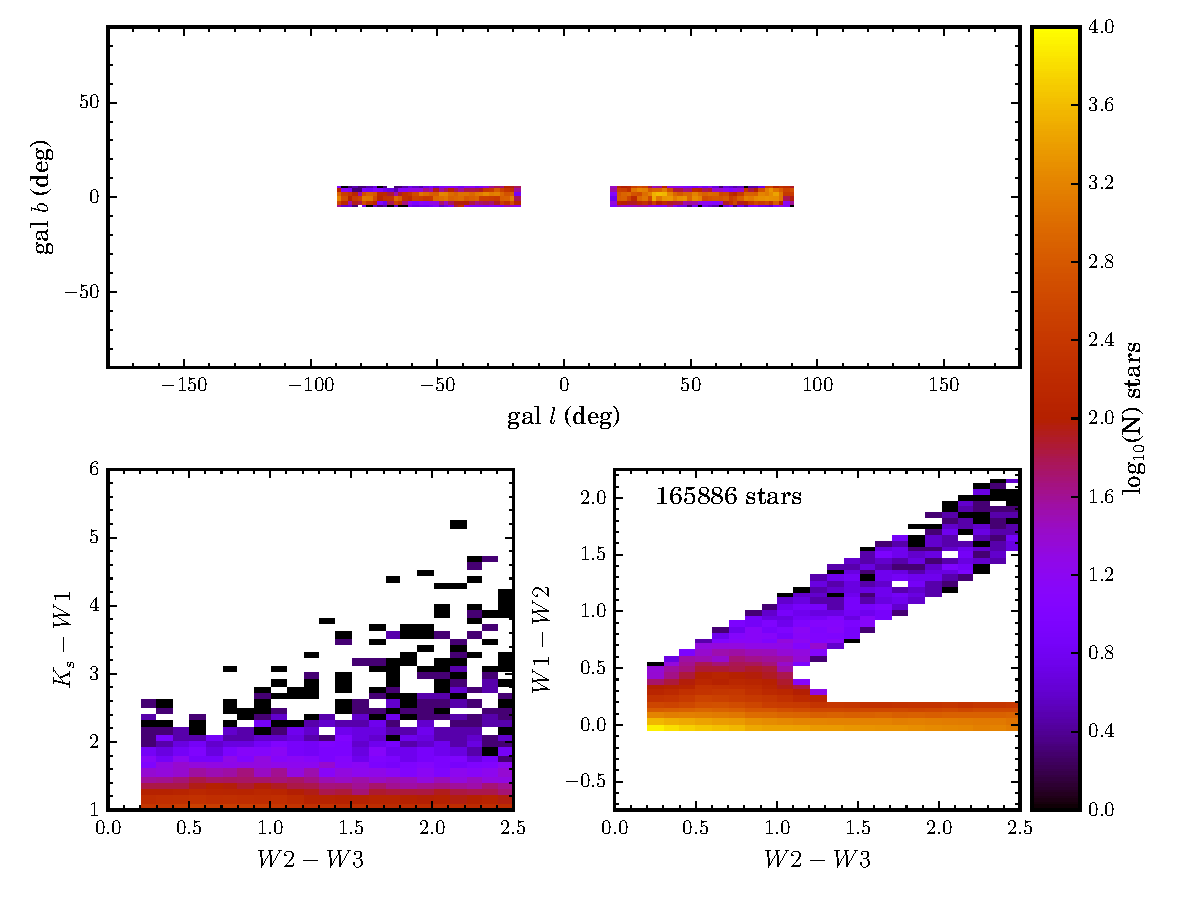
\includegraphics[width=6.5in]{figs/color_and_map_candidates_region1.pdf}
\caption{\label{fig:color_map_candidates1}}
\end{figure}

\begin{figure}[h]
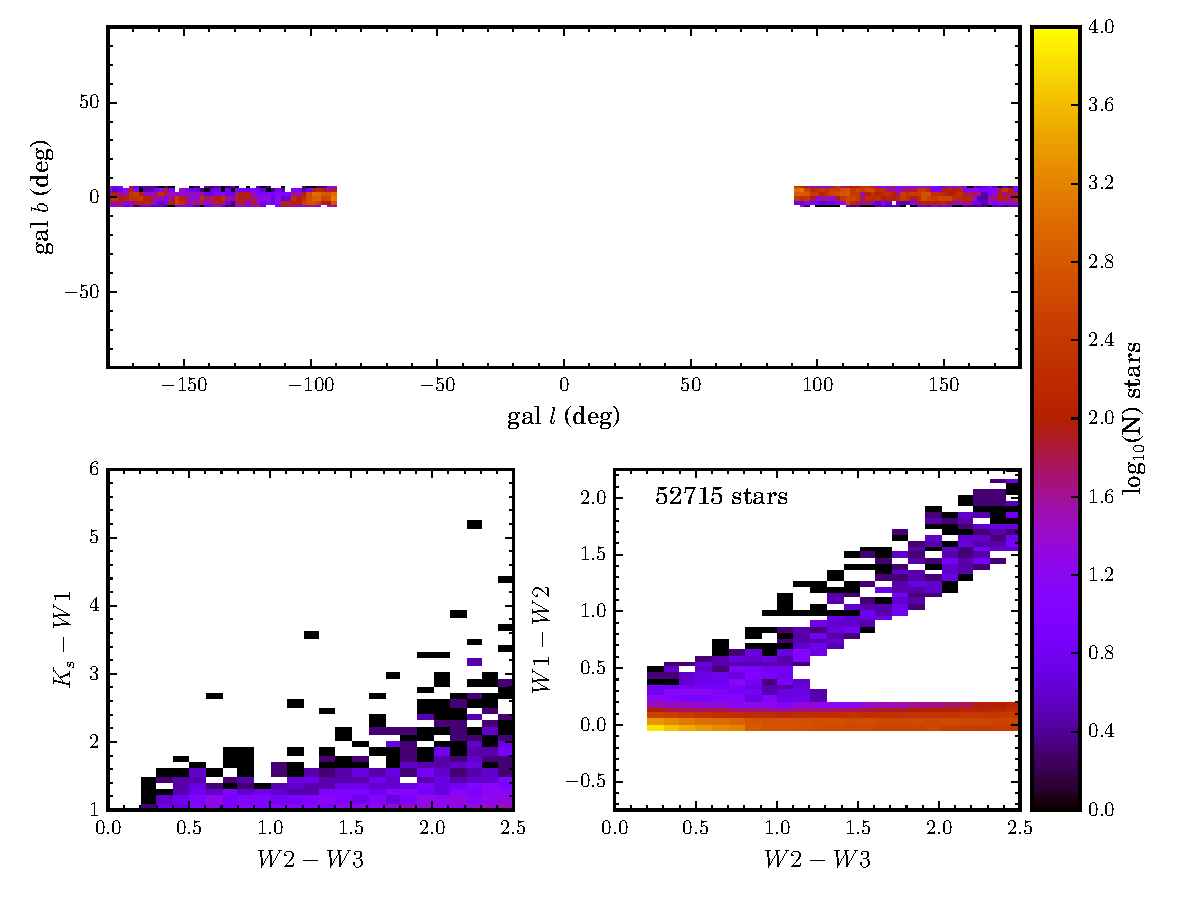
\includegraphics[width=6.5in]{figs/color_and_map_candidates_region2.pdf}
\caption{\label{fig:color_map_candidates2}}
\end{figure}

\begin{figure}[h]
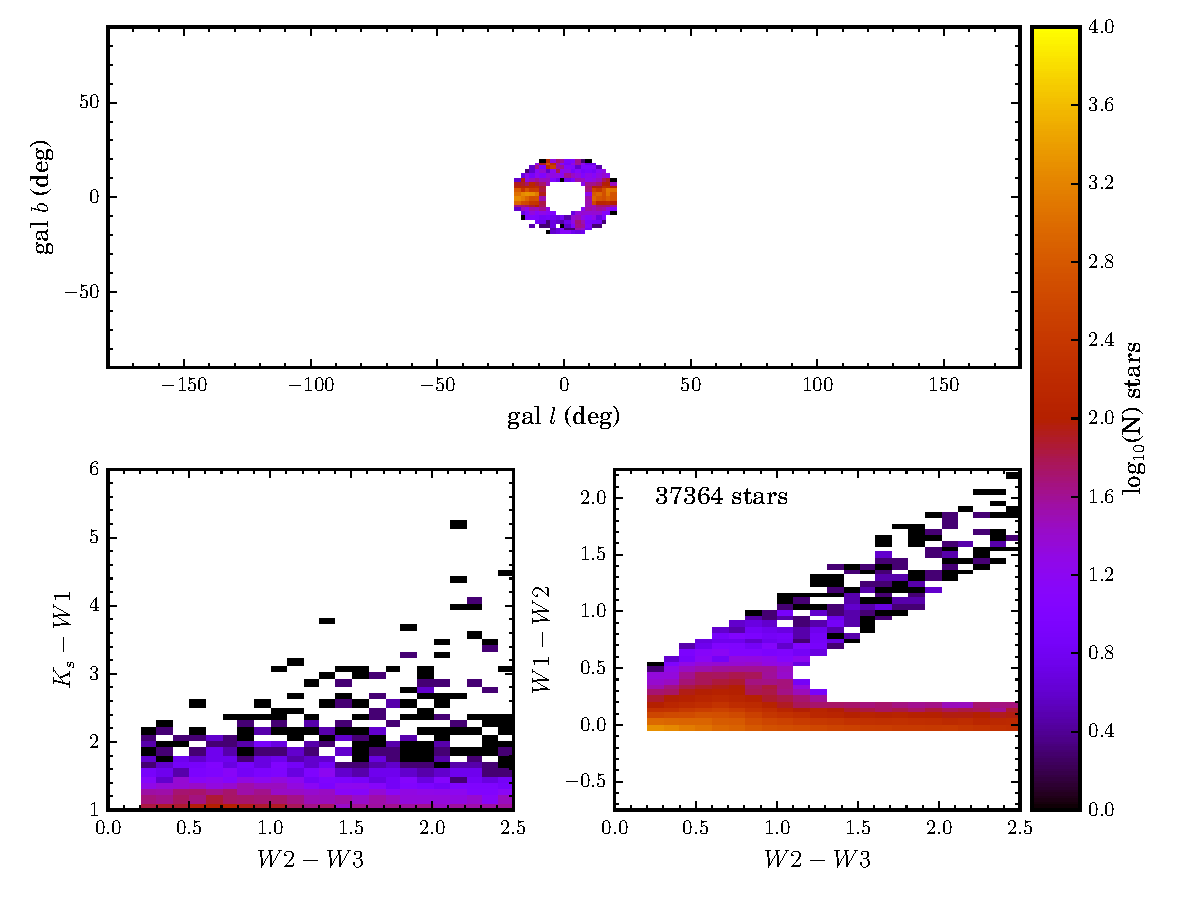
\includegraphics[width=6.5in]{figs/color_and_map_candidates_region3.pdf}
\caption{\label{fig:color_map_candidates3}}
\end{figure}

\begin{figure}[h]
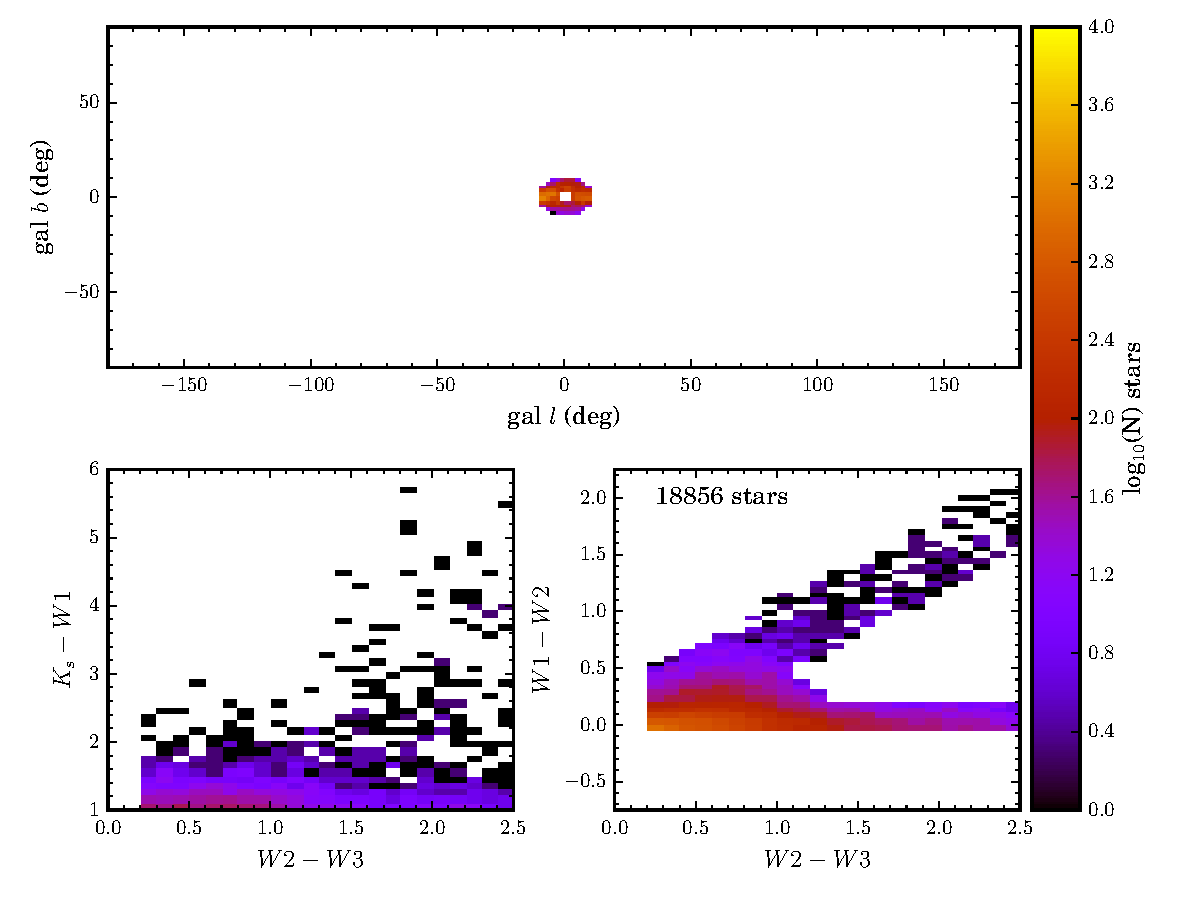
\includegraphics[width=6.5in]{figs/color_and_map_candidates_region4.pdf}
\caption{\label{fig:color_map_candidates4}}
\end{figure}

\begin{figure}[h]
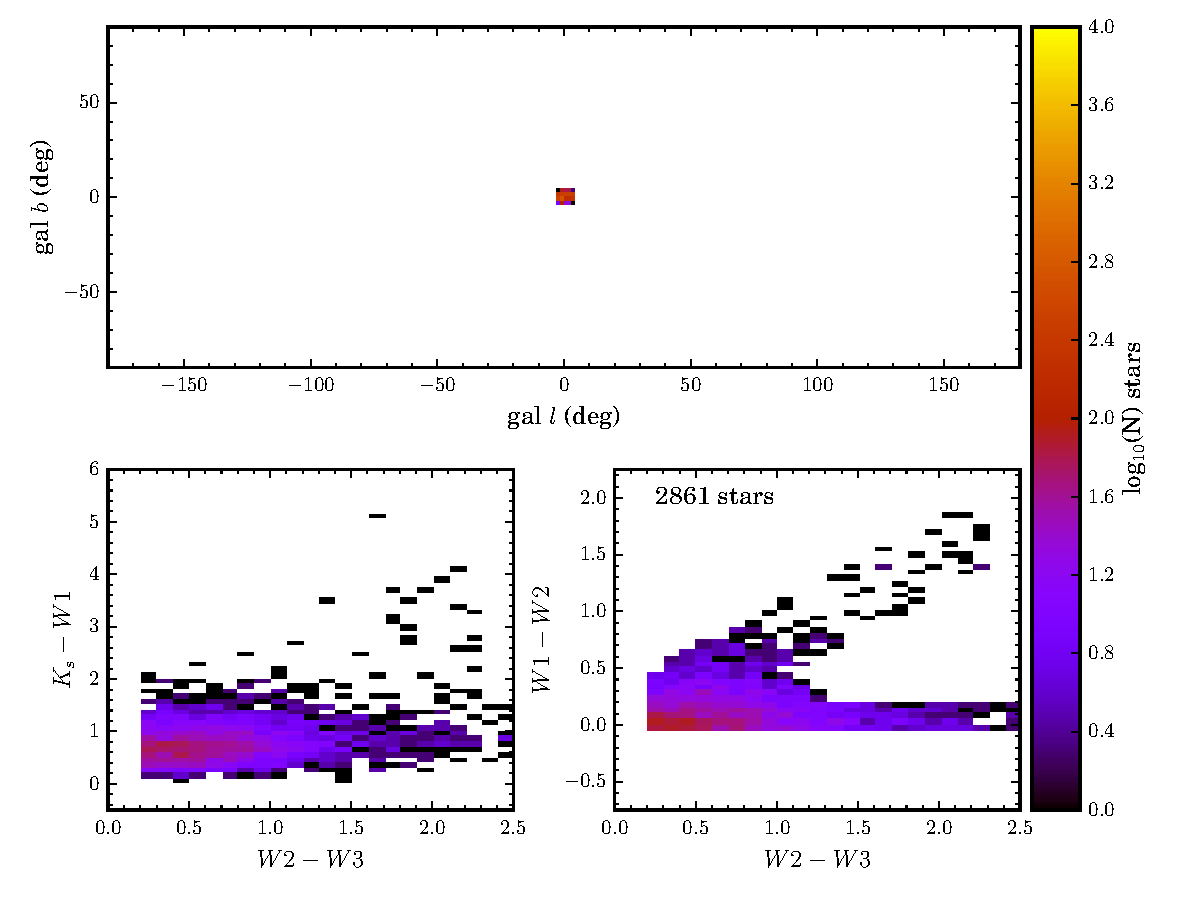
\includegraphics[width=6.5in]{figs/color_and_map_candidates_region5.pdf}
\caption{\label{fig:color_map_candidates5}}
\end{figure}


\subsection{O-rich and C-rich AGB Candidates}
%This section should be somewhat substantial, as you did a lot to get from the previous one through to the end of this one. You used the known AGB stars from OGLE matched to WISE in addition to some help from Nikutta et al 2014 to define O-rich and C-rich boundaries for AGB stars in color-color space. Talk about how these boundaries reduced your sample. Also talk about how these selections of stars were used to estimate  color-magnitude relationships for AGB stars with the LMC as reference, and find some way to justify the 2 magnitude offset that makes the results approach believability. Then talk about how distances were calculated. It was an iterative process that used a test distance to calculate the expected dust column along the line of sight until the sum of distance modulus and extinction coefficient matched apparent minus absolute magnitude. What were the steps in distance modulus? How did you get the extinction coefficient from the color excess that's actually output from galfastdust? What's the source for the galfastdust estimation procedure? And what are the results for the distance measurement?

\subsection{Galactic Number Density}
%This is the section where we show that what we've done is not complete bullshit, though some fecal flecks may remain. The big fig is going to be that plot of |Z| vs. R